% ==============================================================================
% Micro Chapter 3: Supply, Demand, and Market Equilibrium
% Topic alignment: Chiang, Microeconomics (supply and demand chapter). Original text.
% Outcomes: MC-2 (core), C2001-1, C2001-2 (CCSF ECON C2001)
% Review status: DRAFT. Not yet instructor-reviewed (see 02_Pedagogy checklist).
% ==============================================================================
\documentclass[11pt,letterpaper]{article}

% ==============================================================================
% Shared Preamble: Principles of Economics Modular Curriculum
% Core Colors: SlateBlue (#1E293B) & Terracotta (#C2410C)
% ==============================================================================

\usepackage[utf8]{inputenc}
\usepackage[T1]{fontenc}
\usepackage{lmodern}
\usepackage[margin=1in]{geometry}
\usepackage{amsmath,amssymb,amsfonts,amsthm}
\usepackage{booktabs}
\usepackage{microtype}
\usepackage{enumitem}
\usepackage{fancyhdr}
\usepackage{titlesec}
\usepackage{xcolor}
\usepackage{tikz}
\usepackage{pgfplots}
\usepackage{mdframed}
\usepackage[hidelinks,colorlinks=true,linkcolor=SlateBlue,citecolor=SlateBlue,urlcolor=Terracotta]{hyperref}

\pgfplotsset{compat=1.18}
\usetikzlibrary{arrows.meta,positioning,calc,patterns,decorations.pathreplacing}

% --- Color Palette Definitions ---
\definecolor{SlateBlue}{HTML}{1E293B}      % Primary Accent / Structure
\definecolor{Terracotta}{HTML}{C2410C}     % Secondary Accent / Emphasis
\definecolor{ForestGreen}{HTML}{15803D}    % Equilibrium / Positive Shocks
\definecolor{LightSlate}{HTML}{F8FAFC}     % Box Background Fill
\definecolor{BorderGray}{HTML}{CBD5E1}     % Neutral Borders
\definecolor{LightTerracotta}{HTML}{FFF7ED}% Cautionary / Principle Fill

% --- Section Heading Styling ---
\titleformat{\section}
  {\normalfont\Large\bfseries\color{SlateBlue}}{\thesection}{1em}{}[\titlerule]
\titleformat{\subsection}
  {\normalfont\large\bfseries\color{SlateBlue}}{\thesubsection}{1em}{}
\titleformat{\subsubsection}
  {\normalfont\normalsize\bfseries\color{Terracotta}}{\thesubsubsection}{1em}{}

% --- Header and Footer Configuration ---
\pagestyle{fancy}
\fancyhf{}
\renewcommand{\headrulewidth}{0.4pt}
\renewcommand{\footrulewidth}{0.4pt}
\fancyhead[L]{\small\scshape\color{SlateBlue}\leftmark}
\fancyhead[R]{\small\color{SlateBlue}Principles of Economics}
\fancyfoot[C]{\thepage}

% --- Custom Environments (mdframed) ---

% 1. Core Principle Box
\newmdenv[
  linecolor=Terracotta,
  linewidth=1.5pt,
  backgroundcolor=LightTerracotta,
  innertopmargin=10pt,
  innerbottommargin=10pt,
  innerrightmargin=12pt,
  innerleftmargin=12pt,
  roundcorner=4pt,
  skipabove=12pt,
  skipbelow=12pt
]{coreprinciple}

% 2. Empirical Case Study Box
\newmdenv[
  linecolor=SlateBlue,
  linewidth=1.5pt,
  backgroundcolor=LightSlate,
  innertopmargin=10pt,
  innerbottommargin=10pt,
  innerrightmargin=12pt,
  innerleftmargin=12pt,
  roundcorner=4pt,
  skipabove=12pt,
  skipbelow=12pt
]{casestudy}

% 3. Key Takeaways Box
\newmdenv[
  linecolor=BorderGray,
  linewidth=1pt,
  backgroundcolor=white,
  innertopmargin=10pt,
  innerbottommargin=10pt,
  innerrightmargin=12pt,
  innerleftmargin=12pt,
  roundcorner=4pt,
  skipabove=12pt,
  skipbelow=12pt
]{takeaways}

% Environment Title Helpers
\newcommand{\boxheader}[2]{{\noindent\bfseries\color{#1}\Large #2}\vspace{0.4em}\par}
\usepackage{tikz}
\usepackage{pgfplots}
\pgfplotsset{compat=1.18}
\usetikzlibrary{arrows.meta,positioning,calc,shapes.geometric,patterns,decorations.pathreplacing,intersections}

\tikzset{
  econ axis/.style={->, >=Stealth, thick, color=SlateBlue!90!black},
  econ grid/.style={thin, dashed, color=gray!30},
  econ guide/.style={dashed, color=gray!60, thin},
  demand curve/.style={very thick, color=SlateBlue},
  supply curve/.style={very thick, color=Terracotta},
  mb curve/.style={very thick, color=SlateBlue},
  mc curve/.style={very thick, color=Terracotta},
  econ point/.style={circle, fill=SlateBlue!90!black, inner sep=1.8pt},
  econ highlight/.style={fill=Terracotta!20, opacity=0.5},
  econ label/.style={font=\small\sffamily, align=center},
  econ annotation/.style={font=\footnotesize\itshape, color=SlateBlue!80!black}
}


\begin{document}

\title{\Huge\bfseries\color{SlateBlue} Chapter 3: Supply, Demand, and Market Equilibrium}
\author{\large Principles of Microeconomics}
\date{}
\maketitle

\thispagestyle{plain}

\section*{Learning Outcomes}

By the end of this chapter, you will be able to:
\begin{enumerate}[label=\textbf{LO\arabic*.}]
  \item \textbf{Differentiate} a shift of a demand or supply curve from a movement along it, and name the cause of each. \emph{(MC-2, C2001-1, C2001-2)}
  \item \textbf{Calculate} the equilibrium price and quantity from linear demand and supply equations. \emph{(MC-2, C2001-1, C2001-2)}
  \item \textbf{Predict} how equilibrium price and quantity change when demand, supply, or both shift. \emph{(MC-2, C2001-1, C2001-2)}
\end{enumerate}

\tableofcontents
\vspace{1em}
\hrule
\vspace{1em}

% ==============================================================================
\section{Demand}
% ==============================================================================

\subsection{The story}

Think about your own coffee habit. If your favorite caf\'e raises the price of a latte from \$4 to \$6, you probably buy fewer lattes. You might make coffee at home, or switch to a cheaper drink. Now suppose the price stays at \$4, but you get a raise at work and start buying more lattes. In both cases your coffee purchases changed, but the reasons are completely different. The first is a response to the \emph{price of the good}. The second is a response to something \emph{other than that price}. Keeping these two reasons apart is the most important skill in this chapter.

\subsection{The graph}

Put the price, $P$, on the vertical axis and the quantity demanded, $Q$, on the horizontal axis. The \textbf{demand curve} slopes downward: the lower the price, the larger the quantity buyers want to purchase, holding everything else constant. Choose any price on the vertical axis and read across to the curve, then down to the quantity axis. That is the \textbf{quantity demanded} at that price.

\begin{figure}[h]
\centering
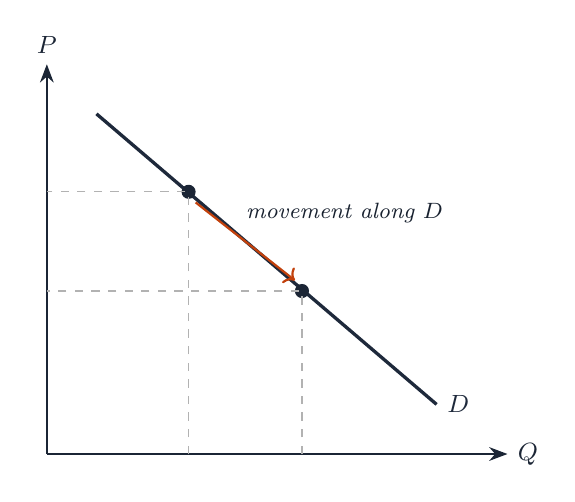
\begin{tikzpicture}[scale=0.9]
  \draw[econ axis] (0,0) -- (6.5,0) node[right, econ label] {$Q$};
  \draw[econ axis] (0,0) -- (0,5.5) node[above, econ label] {$P$};
  \draw[demand curve] (0.7,4.8) -- (5.5,0.7) node[right, econ label] {$D$};
  \node[econ point] at (2.0,3.7) {};
  \node[econ point] at (3.6,2.3) {};
  \draw[econ guide] (2.0,0) -- (2.0,3.7) -- (0,3.7);
  \draw[econ guide] (3.6,0) -- (3.6,2.3) -- (0,2.3);
  \draw[->, thick, color=Terracotta] (2.1,3.55) -- (3.5,2.45);
  \node[econ annotation] at (4.2,3.4) {movement along $D$};
\end{tikzpicture}
\caption{A fall in the price moves buyers down along the same demand curve.}
\end{figure}

\subsection{The math}

A linear demand curve can be written as
\begin{equation}
  Q_d = a - bP, \qquad a>0,\; b>0.
\end{equation}
Here $a$ is the quantity demanded if the price were zero, and $b$ measures how many units of quantity demanded are lost when the price rises by one dollar. The negative sign on $bP$ is the law of demand. Solving for $P$ gives the form that is graphed with $P$ on the vertical axis:
\begin{equation}
  P = \frac{a - Q_d}{b}.
\end{equation}

\subsection{Movement along versus shift of demand}

\begin{coreprinciple}
\boxheader{Terracotta}{Clear It Up: Change in Demand vs. Change in Quantity Demanded}
A change in the \textbf{price of the good itself} moves buyers \emph{along} the demand curve. This is a change in \textbf{quantity demanded}.

A change in any \textbf{non-price determinant} moves the \emph{entire curve}. This is a change in \textbf{demand}. In the equation, this means $a$ changes.

Common mistake: ``The price rose, so demand fell.'' Correct statement: the price rose, so the \emph{quantity demanded} fell.
\end{coreprinciple}

The non-price determinants of demand are:
\begin{itemize}
  \item \textbf{Income.} For a \textbf{normal good}, higher income raises demand. For an \textbf{inferior good}, higher income lowers demand.
  \item \textbf{Prices of related goods.} If the price of a \textbf{substitute} rises, demand for this good rises. If the price of a \textbf{complement} rises, demand for this good falls.
  \item \textbf{Tastes and preferences.}
  \item \textbf{Expectations} about future prices or income.
  \item \textbf{Number of buyers.}
\end{itemize}

An increase in demand shifts the curve to the right: at every price, buyers want more. A decrease shifts it to the left. In the linear model, an increase in demand is an increase in $a$.

% ==============================================================================
\section{Supply}
% ==============================================================================

\subsection{The story}

Consider a roaster that buys green coffee beans, roasts them, and sells the result. If the market price of roasted coffee rises, the roaster earns more on each bag and has a reason to produce more. If instead a drought makes beans more expensive, producing coffee costs more at every level of output, and the roaster will offer fewer bags at any given price. Again there are two different reasons for a change: the \emph{price of the good} versus \emph{everything else}.

\subsection{The graph}

The \textbf{supply curve} slopes upward: the higher the price, the larger the quantity sellers are willing to offer, holding everything else constant. Reading from a price across to the curve and down gives the \textbf{quantity supplied}.

\subsection{The math}

A linear supply curve can be written as
\begin{equation}
  Q_s = c + dP, \qquad d>0.
\end{equation}
Here $d$ measures how much quantity supplied rises when the price rises by one dollar. The intercept $c$ captures everything that is not the price. In many examples $c$ is positive, but it can be zero or negative.

\subsection{Movement along versus shift of supply}

A change in the good's own price moves sellers along the supply curve. A change in a non-price determinant shifts the curve. These determinants include:
\begin{itemize}
  \item \textbf{Input prices} (beans, labor, energy, shipping).
  \item \textbf{Technology.}
  \item \textbf{Number of sellers.}
  \item \textbf{Expectations} about future prices.
  \item \textbf{Taxes, subsidies, and regulations.}
  \item \textbf{Weather} for agricultural goods.
\end{itemize}
An increase in supply shifts the curve to the right, which is an increase in $c$. A decrease in supply shifts it to the left, which is a decrease in $c$.

% ==============================================================================
\section{Market Equilibrium}
% ==============================================================================

\subsection{The story}

A market is where buyers and sellers meet. If the price is too low, buyers want more than sellers offer, so buyers compete and the price rises. If the price is too high, sellers cannot sell everything they produce, so sellers cut the price. The price settles where the quantity buyers want equals the quantity sellers offer.

\subsection{The graph}

The \textbf{equilibrium} is the point where the demand and supply curves cross. At the \textbf{equilibrium price}, $P^*$, quantity demanded equals quantity supplied at the \textbf{equilibrium quantity}, $Q^*$. At a price below $P^*$, there is a \textbf{shortage} ($Q_d>Q_s$). At a price above $P^*$, there is a \textbf{surplus} ($Q_s>Q_d$).

\begin{figure}[h]
\centering
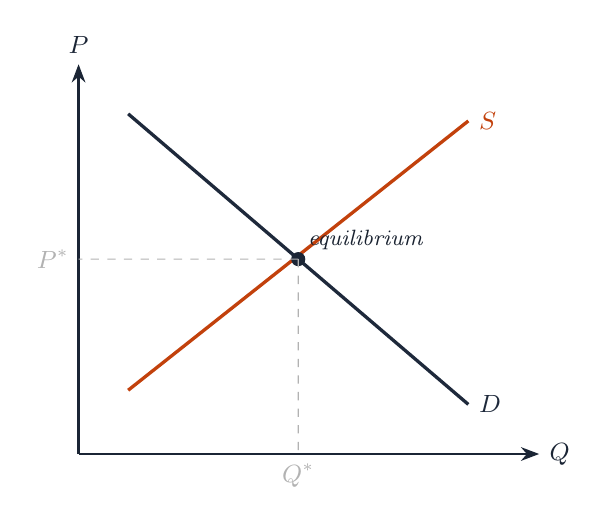
\begin{tikzpicture}[scale=0.9]
  \draw[econ axis] (0,0) -- (6.5,0) node[right, econ label] {$Q$};
  \draw[econ axis] (0,0) -- (0,5.5) node[above, econ label] {$P$};
  \draw[demand curve] (0.7,4.8) -- (5.5,0.7) node[right, econ label] {$D$};
  \draw[supply curve] (0.7,0.9) -- (5.5,4.7) node[right, econ label] {$S$};
  \coordinate (E) at (3.1,2.75);
  \node[econ point] at (E) {};
  \draw[econ guide] (E) -- (3.1,0) node[below, econ label] {$Q^*$};
  \draw[econ guide] (E) -- (0,2.75) node[left, econ label] {$P^*$};
  \node[econ annotation, above right] at (E) {equilibrium};
\end{tikzpicture}
\caption{Equilibrium occurs where demand and supply intersect.}
\end{figure}

\subsection{The math}

Set quantity demanded equal to quantity supplied:
\begin{equation}
  a - bP^* = c + dP^*.
\end{equation}
Collect the price terms on one side:
\begin{equation}
  a - c = (b + d)P^*.
\end{equation}
Solve for the equilibrium price:
\begin{equation}
  P^* = \frac{a - c}{b + d}.
\end{equation}
Substitute $P^*$ into the demand curve to find the equilibrium quantity:
\begin{equation}
  Q^* = a - b\left(\frac{a-c}{b+d}\right) = \frac{ad + bc}{b + d}.
\end{equation}

\begin{casestudy}
\boxheader{SlateBlue}{Worked Example}
Let demand be $Q_d = 120 - 4P$ and supply be $Q_s = 20 + 6P$. Here $a=120$, $b=4$, $c=20$, $d=6$.
\begin{align*}
  P^* &= \frac{120-20}{4+6} = 10,\\
  Q^* &= 120 - 4(10) = 80.
\end{align*}
\textbf{Check:} $Q_s = 20 + 6(10) = 80 = Q_d$. \checkmark

At $P=8$: $Q_d = 88$ and $Q_s = 68$, so there is a shortage of $20$.\\
At $P=12$: $Q_d = 72$ and $Q_s = 92$, so there is a surplus of $20$.
\end{casestudy}

% ==============================================================================
\section{Changes in Equilibrium}
% ==============================================================================

\subsection{The story}

Return to the coffee market. A frost damages the harvest, and coffee becomes scarcer. Or a study reports health benefits of coffee, and more people want it. Each event changes one side of the market, and the price and quantity adjust to a new equilibrium. The order of reasoning never changes: (1) which curve is affected, (2) which direction does it shift, (3) what happens at the new intersection.

\subsection{The graph}

Four single-shift cases, starting from the equilibrium above:

\begin{center}
\begin{tabular}{@{}llcc@{}}
\toprule
\textbf{Event} & \textbf{Curve that shifts} & \textbf{$P^*$} & \textbf{$Q^*$} \\
\midrule
Demand increases & $D$ shifts right & rises & rises \\
Demand decreases & $D$ shifts left & falls & falls \\
Supply increases & $S$ shifts right & falls & rises \\
Supply decreases & $S$ shifts left & rises & falls \\
\bottomrule
\end{tabular}
\end{center}

When \emph{both} curves shift, one effect is certain and the other is ambiguous unless you know which shift is larger.

\begin{center}
\begin{tabular}{@{}lcc@{}}
\toprule
\textbf{Event} & \textbf{$P^*$} & \textbf{$Q^*$} \\
\midrule
Demand increases and supply increases & ambiguous & rises \\
Demand decreases and supply decreases & ambiguous & falls \\
Demand increases and supply decreases & rises & ambiguous \\
Demand decreases and supply increases & falls & ambiguous \\
\bottomrule
\end{tabular}
\end{center}

\subsection{The math}

Because $P^*=(a-c)/(b+d)$ and $Q^*=(ad+bc)/(b+d)$, how the equilibrium responds to a shift follows directly:
\begin{align}
  \frac{\partial P^*}{\partial a} &= \frac{1}{b+d} > 0, &
  \frac{\partial Q^*}{\partial a} &= \frac{d}{b+d} > 0,\\
  \frac{\partial P^*}{\partial c} &= -\frac{1}{b+d} < 0, &
  \frac{\partial Q^*}{\partial c} &= \frac{b}{b+d} > 0.
\end{align}
An increase in demand ($a$ up) raises both $P^*$ and $Q^*$. An increase in supply ($c$ up) lowers $P^*$ and raises $Q^*$. These match the table.

\begin{casestudy}
\boxheader{SlateBlue}{Worked Example: Shifts in Both Directions}
Start from $Q_d = 120 - 4P$ and $Q_s = 20 + 6P$, with $P^*=10$ and $Q^*=80$.

\begin{center}
\begin{tabular}{@{}lccc@{}}
\toprule
\textbf{Change} & \textbf{New equation} & \textbf{$P^*$} & \textbf{$Q^*$} \\
\midrule
Demand rises ($a=160$) & $Q_d=160-4P$ & $14$ & $104$ \\
Supply falls ($c=0$) & $Q_s=0+6P$ & $12$ & $72$ \\
Both: $a=160$, $c=0$ & both changed & $16$ & $96$ \\
\bottomrule
\end{tabular}
\end{center}
In the last row the price rises for sure, and in this case quantity also rises because the demand shift is larger. If the supply shift had been larger, quantity would have fallen.
\end{casestudy}

% ==============================================================================
\section{Evidence: Coffee Prices in the Data}
% ==============================================================================

The Federal Reserve Bank of St.\ Louis publishes the International Monetary Fund's monthly benchmark for the global price of Arabica coffee. The series code is \textbf{PCOFFOTMUSDM}, titled \emph{Global price of Coffee, Other Mild Arabica}, measured in U.S.\ cents per pound, monthly, not seasonally adjusted. Find it at \url{https://fred.stlouisfed.org/series/PCOFFOTMUSDM}.

\begin{coreprinciple}
\boxheader{Terracotta}{Nominal vs. Real}
This series is a \textbf{nominal} price. It is not adjusted for inflation. A rising nominal price does not by itself show that coffee became more expensive relative to other goods. To compare across years, divide by a price index (for example, the CPI series \textbf{CPIAUCSL}) to get a \textbf{real} price.
\end{coreprinciple}

\textbf{Discussion.} Pick a period when this series moved sharply. Name one demand-side and one supply-side event that could explain it. Which curve shifted, in which direction, and what does your story predict for the quantity traded? Why can the price series alone not tell you which story is right?

% ==============================================================================
\section{Practice Problems}
% ==============================================================================

\begin{enumerate}[label=\textbf{\arabic*.}]
  \item Demand is $Q_d = 200 - 5P$ and supply is $Q_s = 50 + 10P$. Find $P^*$ and $Q^*$.
  \item In the market from Problem 1, demand rises to $Q_d = 230 - 5P$. Find the new $P^*$ and $Q^*$. Is this a shift or a movement?
  \item For each event, state whether the coffee \emph{demand} curve shifts, the \emph{supply} curve shifts, or there is a movement along a curve, and give the direction.
  \begin{enumerate}[label=(\alph*)]
    \item The price of tea, a substitute, rises.
    \item A frost destroys part of the harvest.
    \item The price of coffee rises, and buyers purchase less.
    \item A new roasting machine lowers costs.
  \end{enumerate}
\end{enumerate}

\subsection*{Solutions}
\begin{enumerate}[label=\textbf{\arabic*.}]
  \item $P^* = \dfrac{200-50}{5+10} = 10$ and $Q^* = 200 - 5(10) = 150$. Check: $Q_s = 50 + 100 = 150$. \checkmark
  \item $P^* = \dfrac{230-50}{15} = 12$ and $Q^* = 230 - 5(12) = 170$. Check: $Q_s = 50 + 120 = 170$. \checkmark This is a \textbf{shift} of the demand curve (the intercept $a$ changed from $200$ to $230$). The rise in price from $10$ to $12$ is a \textbf{movement along} the supply curve.
  \item (a) Demand shifts right. (b) Supply shifts left. (c) Movement along the demand curve (a decrease in quantity demanded). (d) Supply shifts right.
\end{enumerate}

\begin{takeaways}
\boxheader{SlateBlue}{Key Takeaways}
\begin{itemize}
  \item Own price changes cause \textbf{movements along} a curve. Non-price determinants cause \textbf{shifts}.
  \item In $Q_d=a-bP$ and $Q_s=c+dP$, shifts change $a$ or $c$. Movements change $P$.
  \item $P^* = \dfrac{a-c}{b+d}$ and $Q^* = \dfrac{ad+bc}{b+d}$.
  \item One curve shifts: the effect on $P^*$ and $Q^*$ is certain. Both shift: one effect is ambiguous.
  \item Nominal prices are not adjusted for inflation. Use a price index to get real prices.
\end{itemize}
\end{takeaways}

\end{document}
